\documentclass[journal,12pt,twocolumn]{IEEEtran}

\usepackage{setspace}
\usepackage{gensymb}

\singlespacing


\usepackage[cmex10]{amsmath}

\usepackage{amsthm}

\usepackage{mathrsfs}
\usepackage{txfonts}
\usepackage{stfloats}
\usepackage{bm}
\usepackage{cite}
\usepackage{cases}
\usepackage{subfig}

\usepackage{longtable}
\usepackage{multirow}

\usepackage{enumitem}
\usepackage{mathtools}
\usepackage{steinmetz}
\usepackage{tikz}
\usepackage{circuitikz}
\usepackage{verbatim}
\usepackage{tfrupee}
\usepackage[breaklinks=true]{hyperref}
\usepackage{graphicx}
\usepackage{tkz-euclide}
\usepackage{float}

\usetikzlibrary{calc,math}
\usepackage{listings}
    \usepackage{color}                                            %%
    \usepackage{array}                                            %%
    \usepackage{longtable}                                        %%
    \usepackage{calc}                                             %%
    \usepackage{multirow}                                         %%
    \usepackage{hhline}                                           %%
    \usepackage{ifthen}                                           %%
    \usepackage{lscape}     
\usepackage{multicol}
\usepackage{chngcntr}

\DeclareMathOperator*{\Res}{Res}

\renewcommand\thesection{\arabic{section}}
\renewcommand\thesubsection{\thesection.\arabic{subsection}}
\renewcommand\thesubsubsection{\thesubsection.\arabic{subsubsection}}

\renewcommand\thesectiondis{\arabic{section}}
\renewcommand\thesubsectiondis{\thesectiondis.\arabic{subsection}}
\renewcommand\thesubsubsectiondis{\thesubsectiondis.\arabic{subsubsection}}


\hyphenation{op-tical net-works semi-conduc-tor}
\def\inputGnumericTable{}                                 %%

\lstset{
%language=C,
frame=single, 
breaklines=true,
columns=fullflexible
}
\begin{document}


\newtheorem{theorem}{Theorem}[section]
\newtheorem{problem}{Problem}
\newtheorem{proposition}{Proposition}[section]
\newtheorem{lemma}{Lemma}[section]
\newtheorem{corollary}[theorem]{Corollary}
\newtheorem{example}{Example}[section]
\newtheorem{definition}[problem]{Definition}

\newcommand{\BEQA}{\begin{eqnarray}}
\newcommand{\EEQA}{\end{eqnarray}}
\newcommand{\define}{\stackrel{\triangle}{=}}
\newcommand\hlight[1]{\tikz[overlay, remember picture,baseline=-\the\dimexpr\fontdimen22\textfont2\relax]\node[rectangle,fill=blue!50,rounded corners,fill opacity = 0.2,draw,thick,text opacity =1] {$#1$};}
\bibliographystyle{IEEEtran}
\providecommand{\mbf}{\mathbf}
\providecommand{\pr}[1]{\ensuremath{\Pr\left(#1\right)}}
\providecommand{\qfunc}[1]{\ensuremath{Q\left(#1\right)}}
\providecommand{\sbrak}[1]{\ensuremath{{}\left[#1\right]}}
\providecommand{\lsbrak}[1]{\ensuremath{{}\left[#1\right.}}
\providecommand{\rsbrak}[1]{\ensuremath{{}\left.#1\right]}}
\providecommand{\brak}[1]{\ensuremath{\left(#1\right)}}
\providecommand{\lbrak}[1]{\ensuremath{\left(#1\right.}}
\providecommand{\rbrak}[1]{\ensuremath{\left.#1\right)}}
\providecommand{\cbrak}[1]{\ensuremath{\left\{#1\right\}}}
\providecommand{\lcbrak}[1]{\ensuremath{\left\{#1\right.}}
\providecommand{\rcbrak}[1]{\ensuremath{\left.#1\right\}}}
\theoremstyle{remark}
\newtheorem{rem}{Remark}
\newcommand{\sgn}{\mathop{\mathrm{sgn}}}
\providecommand{\abs}[1]{\left\vert#1\right\vert}
\providecommand{\res}[1]{\Res\displaylimits_{#1}} 
\providecommand{\norm}[1]{$\left\lVert#1\right\rVert$}
%\providecommand{\norm}[1]{\lVert#1\rVert}
\providecommand{\mtx}[1]{\mathbf{#1}}
\providecommand{\mean}[1]{E\left[ #1 \right]}
\providecommand{\fourier}{\overset{\mathcal{F}}{ \rightleftharpoons}}
%\providecommand{\hilbert}{\overset{\mathcal{H}}{ \rightleftharpoons}}
\providecommand{\system}{\overset{\mathcal{H}}{ \longleftrightarrow}}
	%\newcommand{\solution}[2]{\textbf{Solution:}{#1}}
\newcommand{\solution}{\noindent \textbf{Solution: }}
\newcommand{\cosec}{\,\text{cosec}\,}
\providecommand{\dec}[2]{\ensuremath{\overset{#1}{\underset{#2}{\gtrless}}}}
\newcommand{\myvec}[1]{\ensuremath{\begin{pmatrix}#1\end{pmatrix}}}
\newcommand{\mydet}[1]{\ensuremath{\begin{vmatrix}#1\end{vmatrix}}}
\numberwithin{equation}{subsection}
\makeatletter
\@addtoreset{figure}{problem}
\makeatother
\let\StandardTheFigure\thefigure
\let\vec\mathbf
\renewcommand{\thefigure}{\theproblem}
\def\putbox#1#2#3{\makebox[0in][l]{\makebox[#1][l]{}\raisebox{\baselineskip}[0in][0in]{\raisebox{#2}[0in][0in]{#3}}}}
     \def\rightbox#1{\makebox[0in][r]{#1}}
     \def\centbox#1{\makebox[0in]{#1}}
     \def\topbox#1{\raisebox{-\baselineskip}[0in][0in]{#1}}
     \def\midbox#1{\raisebox{-0.5\baselineskip}[0in][0in]{#1}}
\vspace{3cm}
\title{Assignment No.2}
\author{Valli Devi Bolla}
\maketitle
\newpage
\bigskip
\renewcommand{\thefigure}{\theenumi}
\renewcommand{\thetable}{\theenumi}
Download all python codes from 
\begin{lstlisting}
https://github.com/Vallidevibolla/Assignment-2-1/blob/main/code.py
\end{lstlisting}
%
and latex-tikz codes from 
%
\begin{lstlisting}
https://github.com/Vallidevibolla/Assignment-2-1/blob/main/main.tex
\end{lstlisting}
%
Question taken from
\begin{lstlisting}
https://github.com/gadepall/ncert/blob/main/linalg/vectors/gvv_ncert_vectors.pdf- Q.no.2.25 
\end{lstlisting}
%
\section{Question No.2.25}
Find a point on the y-axis which is equidistant from the points A=\myvec{6\\5} and B=\myvec{-4\\3}
\section{Solution}
Given, 
\begin{align}
\vec{A}=\myvec{6\\5} \\
\vec{B}=\myvec{-4\\3}
\end{align}
Let $\underline{x}$ be the point on y-axis.Then\\
\begin{align}
//$\underline{x}$-\vec{A}//^2=//$\underline{x}$-\vec{B}//^2
\\
\boxed{($\underline{x}$-\vec{A})^T($\underline{x}$-\vec{A})=($\underline{x}$-\vec{B})^T($\underline{x}$-\vec{B})}
\\
($\underline{x}$-\vec{A})^T(\vec{x}-\vec{A})=$\underline{x}$^T \vec{x}-$\underline{x}$^T \vec{A}-\vec{A}^T \vec{x}+\vec{A}^T \vec{A}
\\
($\underline{x}$-\vec{B})^T(\vec{x}-\vec{B})=$\underline{x}$^T \vec{x}-$\underline{x}$^T \vec{B}-\vec{B}^T \vec{x}+\vec{B}^T \vec{B}
\end{align}
Consider the expressions 
\begin{align}
\vec{x}^T \vec{x}=//\vec{x}//^2\\
\vec{x}^T \vec{A}=\vec{A}^T \vec{x}
\end{align}
Final expression of equ.2.0.4 using this written as 
\begin{align}
//\vec{x}//^2-2 \vec{A}^T \vec{x}+\vec{A}^T \vec{A}=//\vec{x}//^2-2 \vec{B}^T \vec{x}+\vec{B}^T \vec{B}\\
\implies-2 \vec{A}^T \vec{x}+2 \vec{B}^T \vec{x}= \vec{B}^T \vec{B}-\vec{A}^T \vec{A}\\
\implies 2 \vec{x}(\vec{A}^T-\vec{B}^T)= \vec{A}^T \vec{A}-\vec{B}^T \vec{B}\\
2 \vec{x}(\vec{A}^T-\vec{B}^T)=//\vec{A}//^2-//\vec{B}//^2
\end{align}
\vec{x} lies on the y-axis\\
\vec{{x}} = y\myvec{0\\1}= y \vec{e_2}
Now substitute this in equ.2.0.12
\begin{align}
2\vec{ye_2}\vec{(A^T-B^T)}=\vec{//A//}^2-\vec{//B//}^2\\
\boxed{\vec{y}=$\dfrac{\vec{//A//}^2-\vec{//B//}^2}{\vec{2e_2}.\vec{(A^T-B^T)}}$}\\
\vec{2e_2}.\vec{(A^T-B^T)}=2\myvec{0\\1}.\myvec{10\ 2}=4\\
\implies\vec{y}=\myvec{$\dfrac{61-25}{4}$}
\vec{y}=\myvec{$\dfrac{36}{4}$}\\
 \boxed{$\therefore$ y=9}
\end{align}
     
\numberwithin{figure}{section}
\begin{figure}[ht]
    \centering
    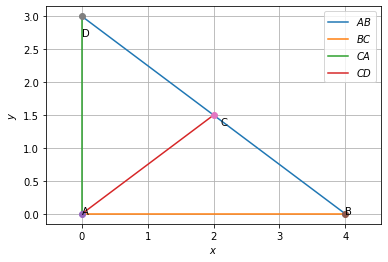
\includegraphics[width=\columnwidth]{download.png}
    \caption{Fig. 2.25}
    \label{Graphical solution}
\end{figure}
\end{document}
